\documentclass{article}
\usepackage{fancyhdr}
\usepackage{lastpage}
\usepackage{amsmath}
\usepackage{amssymb}
\usepackage{amsthm}
\usepackage[margin=1in]{geometry}
\usepackage{graphicx}
\graphicspath{ {./} }

\pagestyle{fancy}
\setlength\headheight{28pt}
\addtolength{\headheight}{\baselineskip}
\fancyhf{}
\renewcommand{\headrulewidth}{0pt}
\lhead{Math 251 - Shuichi Masuda\\Juno Suárez\\\today}
\rfoot{Page \thepage \hspace{1pt} of \pageref{LastPage}}

\renewcommand\thesubsection{\arabic{subsection}.}
\renewcommand\thesubsubsection{\alph{subsubsection})}

\begin{document}

\section*{Computer Lab \# 3}

\subsection{}
Prediction:

$$ \lim_{x \rightarrow 0} x^2 sin(\frac{1}{x}) = \boxed{0} $$

Based on two factors: $sin(\frac{1}{x})$ presents a challenge, as $\frac{1}{x}$ will increase in magnitude for values of $x < 1$ as they get closer to 0. If the value of the argument to $sin$ were approaching, say, 0, it would be a good indication, because we could say that $sin(\approx0) \approx 0$. However, since it's instead an arbitrarily large value, and not obviously a multiple of the period of $sin$, it's hard to predict the value of $sin(\frac{1}{x})$ except to say we know it will be in the range of $sin$, $[-1,1]$.

The other factor, however, is $x^2$, so as $x$ approaches 0, $x^2$ will approach 0. Therefore, the overall limit, if it exists, should approach $0$. Since $sin$ and $x^2$ are continuous, I predict that the overall function will be continuous and that the overall limit will exist and approach 0.

\subsection{}
\emph{Step performed in GeoGebra.}

\subsection{}
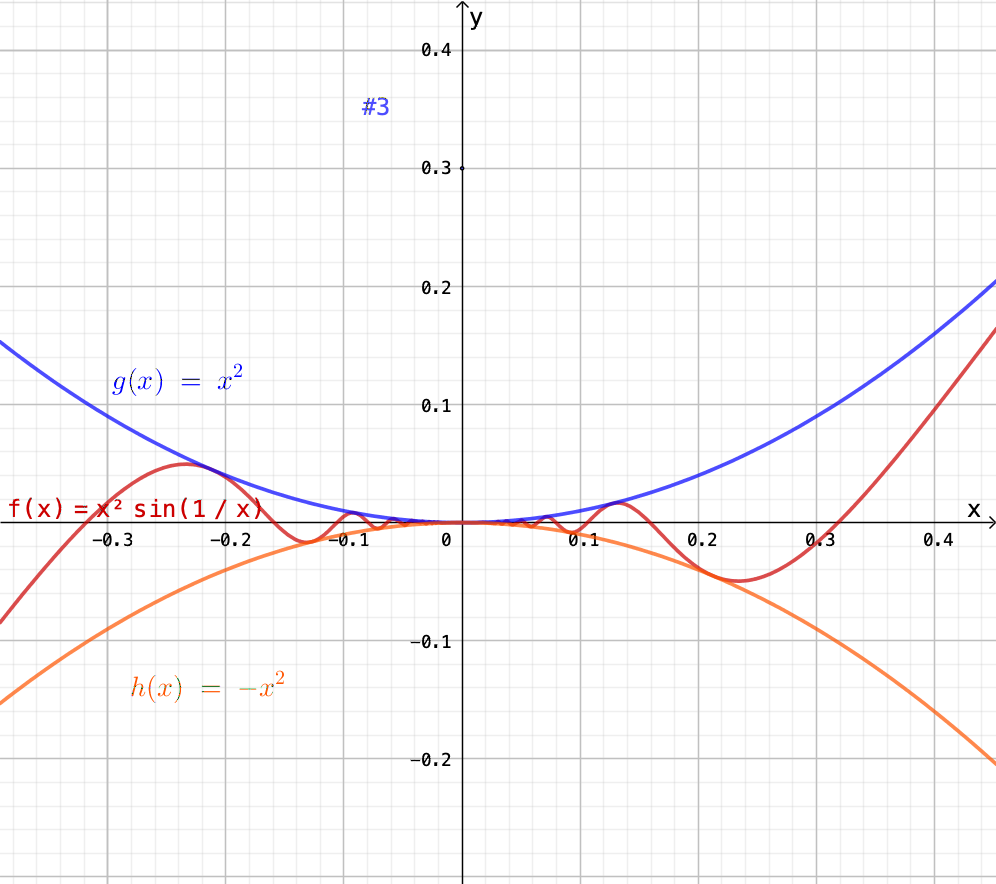
\includegraphics[width=\textwidth]{cl3-3}

\subsection{}
Since $x^2$ and $-x^2$ are continuous, we can find their limits by the substitution method:
$$
\lim_{x \rightarrow 0}x^2 = (0)^2 = \boxed{0}
$$
$$
\lim_{x \rightarrow 0}-x^2 = -(0)^2 = \boxed{0}
$$

\subsection{}
Graphically, it appears that $f(x)=x^2sin(\frac{1}{x})$ is less than or equal to $g(x)=x^2$ for all points in the domain as $x$ approaches 0 from the left and from the right. Further, it appears that $f(x)$ is greater than or equal to $h(x)=-x^2$ on the same interval. Further, we can check our intuition by noticing that $sin$ is a scaling factor of $f(x)$. Since the range of $sin$ is $[-1,1]$, an expression scaled by $sin$ will always be less than or equal to the unscaled term. So the inequality holds.

In \# 4, we evaluated the limits of $g(x)$ and $h(x)$ as $x$ approaches 0.

Therefore, we can say that $f(x)$ is squeezed by $g(x)$ and $h(x)$ as $x$ approaches 0, and we can solve for $\lim_{x \rightarrow 0}f(x)$ using the Squeeze Theorem.

\subsection{}
Via the squeeze theorem, given

$$
h(x) \leq f(x) \leq g(x) \text{  as $x$ approaches 0}
$$
$$
\lim_{x \rightarrow 0}g(x) = (0)^2 = \boxed{0}
$$
$$
\lim_{x \rightarrow 0}h(x) = -(0)^2 = \boxed{0}
$$
and since
$$
\lim_{x \rightarrow 0}g(x) = \lim_{x \rightarrow 0}h(x)
$$
then we can say
$$ \lim_{x \rightarrow 0} x^2 sin(\frac{1}{x}) = \boxed{0} $$

$\hfill \square$


\subsection{}
Considering
$$
f(x) = \frac{sin(x)}{x}
$$

the numeric and graphical investigation in Computer Lab \# 2 suggested
$$
\lim_{x \rightarrow 0} f(x) = \boxed{1}
$$

\subsection{}
\emph{Step performed in GeoGebra.}

\subsection{}
\emph{Step performed in GeoGebra.}

\subsection{}
Two functions that squeeze $f(x)$ near $x=0$ are:
$$g(x)=1$$
$$h(x)=cos(x)$$

The range of $sin$ is $[-1,1]$ so the inequality $f(x) \leq g(x)$ will always hold. For all $x$ near 0, $g(x)$ is graphically less than $f(x)$. It's not the soumdest of mathematical reasoning, but given the periodicity of $sin$ and $cos$ we can have strong confidence that the actual behavior of these functions matches the behavior apparent from the graph.

Both functions are continuous, so we can find their limits by the Substitution Method:
\begin{align}
  \lim_{x \rightarrow 0}g(x) \notag \\
  \boxed{1} \notag
\end{align}

\begin{align}
  \lim_{x \rightarrow 0}h(x) \notag \\
  cos(0) \notag \\
  \boxed{1} \notag
\end{align}

Because the limits of $g(x)$ and $h(x)$ as $x$ approaches 0 are the same, we can say that this value is also the limit of $f(x)$ as $x$ approaches 0, by the Squeeze Theorem. That is,
$$
\lim_{x \rightarrow 0} \frac{sin(x)}{x} = \boxed{1}
$$
$\hfill \square$

\subsection{}
\includegraphics[width=\textwidth]{cl3-11}

\subsection{}
\emph{Step performed in GeoGebra.}



\end{document}
